\documentclass{acm_proc_article-sp}
\usepackage{fancyhdr}
\usepackage{amssymb}
\usepackage{amsmath}
\usepackage{amsfonts}
\usepackage[T1]{fontenc} % get tt fonts to work right
\usepackage{graphicx}
\usepackage{fixltx2e}
\usepackage{multirow}
\usepackage{color}
\usepackage{caption}
\DeclareCaptionType{copyrightbox} % workaround for bug in caption
\usepackage{subcaption}
\usepackage{xspace}
\usepackage{url}
\usepackage{listings}
\usepackage[all]{nowidow}

\begin{document}

\special{papersize=8.5in,11in}
\setlength{\pdfpageheight}{\paperheight}
\setlength{\pdfpagewidth}{\paperwidth}

\definecolor{darkblue}{rgb}{0,0,0.7}
\definecolor{darkgreen}{rgb}{0,0.5,0}
\definecolor{orange}{rgb}{0.7,0.5,0.0}
\definecolor{brown}{rgb}{0.8,0.4,0.0}

\definecolor{teal}{rgb}{0.06,0.3,0.3}
\definecolor{maroon}{rgb}{0.5,0.0,0.25}
\definecolor{darkblue}{rgb}{0.0,0.2,0.75}
\definecolor{darkred}{rgb}{0.7,0.0,0.0}
\definecolor{darkgreen2}{rgb}{0,0.35,0}
\definecolor{darkgreen}{rgb}{0,0.5,0}
\newcommand{\timnote}[1]{ {\textcolor{maroon} { Tim: #1 }}}
\newcommand{\todo}[1]{ {\textcolor{red} { TODO: #1 }}}

%\title{How low can you halo?}
\title{Modeling Halo Exchange on Multi-dimensional Torus Networks}

\numberofauthors{2}

\author{
% 1st. author
\alignauthor
Yadu Nand Babuji\\
       \affaddr{Dept. of Computer Science,}\\
       \affaddr{University of Chicago,}\\
       \affaddr{Chicago, IL, USA}\\
       \email{yadunand@uchicago.edu}
% 2nd. author
\alignauthor
Timothy G. Armstrong\\
       \affaddr{Dept. of Computer Science,}\\
       \affaddr{University of Chicago,}\\
       \affaddr{Chicago, IL, USA}\\
       \email{tga@uchicago.edu}
}
\maketitle

\begin{abstract}
% Motivation
Many High Performance Computing (HPC) applications involve application domain decompositions that involve nearest neighbor communication.
Halo exchange is a common nearest neighbor communication pattern that arises
as a result of domain decomposition and occurs in a wide range of HPC applications.
% Problem statement % Approach
Empirical results show that different task placement strategies in Halo exchange codes can have as much as 7.5x performance difference.
We develop an analytical model to understand the impact of task placements within a network topology on performance and guide selection of
optimal mappings.
% Results
We have identified an optimized mapping which outperform the default mapping 2.68x and several sub-optimal mapping strategies.
Our Analytic model performs within 30\% percentage average error of empirical results with a maximum of 53.6\% under-prediction.
% Conclusions

\end{abstract}

\section{Introduction}

% Intro
Halo exchange is a common communication pattern in parallel codes, where
each process is assigned an application subdomain and must periodically
communicate with other processors that have neighboring subdomains to
update information about the state of the boundary between subdomains~\cite{Kjolstad_2010}.
A common special case is when a multi-dimensional cartesian space is
decomposed into subdomains of equal size.  For example, in the three-dimensional
(3D) case, a 8x8x8 cube might be decomposed into 256 2x1x1 cubes for execution on 256 processors.
Figure~\ref{fig:halo-illustration} illustrates the two-dimensional (2D) case on 8
processors.

\begin{figure}
  \center
  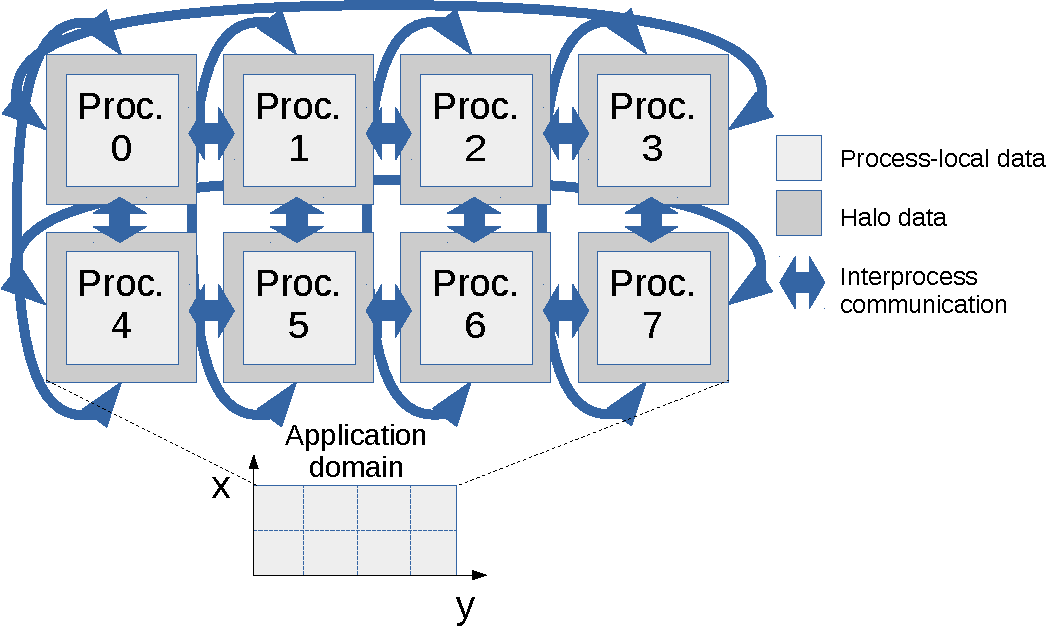
\includegraphics[width=0.475\textwidth]{fig/halo-illustration}
  \caption{Halo exchange for a 2D cartesian domain with wraparound on 8 processors}
    \label{fig:halo-illustration}
\end{figure}

% Objective
This paper explores the problem of mapping such multi-dimensional cartesian
halo exchange communications onto parallel computers with hypercube or
torus networks. A typical computation job on a leadership class machine would
utilize several hundreds to thousands of cores, as a result there are a large number of
possible mappings to the physical hardware that could be chosen. We seek to understand
what aspects of the mappings have an impact on performance and how to quantify the the impact of the mappings on performance. Mapping strategies
are an easy and effective optimization, which require no code changes to the application.  Our empirical studies show that these mapping strategies have significantly
different performance characteristics for network communication.

% Tim: I don't think this is entirely true:
%There are no studies to the best
%of our knowledge that attempts to model the impact of mapping performance on
%HPC systems.

% What does this paper contribute:
The contributions of this paper are the following. We have identified average distance as
a simple yet useful metric by which task placement strategies or mappings can be quantified.
An analytical model for the performance of halo exchange operation is developed which is accurate
to within 30\% error rate. We have also identified eight distinct mapping strategies
which are used to evaluate our model.
Within these are nearly optimal and pessimal mapping strategies, with
the optimal strategy yielding 2x improvement in performance over the default mapping.

The rest of the paper is organised as follows :
% Guidance
The rest of the paper is organised as follows: Section 2, provides background information on
the HPC system topologies and BlueGene/Q in particular. Section 3, describes mapping strategies.
Section 4, develops the analytical model and Section 5, details the experiment design for empirical
validation of the model.

% Summary conclusions

\section{High-Performance Computer Networks}

The state of the art in High Performance Computing(HPC) infrastructure, demands high-performance networks
to support the movement of data between the nodes as well as to-and-from disk-arrays. HPC systems are
increasingly architected with high radix interconnects such as hypercubes and N-dimensional tori.
For HPC applications which involve fine-grained communication,
high-radix networks provide low latency, smaller diameter, and large bandwidth as multiple links along the multiple
dimensions supported.
Parallel applications have a wide range of task placement options that can
exploit the network topology of these HPC systems based on the communication
patterns of the application.
%These networks have evolved to several different network topologies in order to support
%different requirements, and data movement patterns.

% Routing protocols on the BG/Q
% Direct routing
% Adaptive routing
\subsection{Blue Gene/Q 5D Torus Network}

The BlueGene/Q is a massively parallel supercomputer from IBM, the third
generation of the BlueGene series of supercomputers.
The first two generations of BlueGene systems used a three-dimensional
torus network, while the BlueGene/Q uses a five-dimensional (5D) torus with up
to 16K nodes.  
To support the five-dimensional torus each compute node has 10 bi-directional full-duplex links. There is a separate 11th link for IO. Each of the 10 links
operate at a bandwidth of 2GB/s \cite{BGQ_RedBook_2013}. After accounting for 10\% overhead in message headers 1.8GB/s is available for raw data per link in one-direction.
The 5D torus network provides high nearest neighbor and bisection bandwidth
while limiting the maximum number of hops to reach the furthest nodes of
the network and therefore reducing latency. The five dimensions on the
network are labelled as
A,B,C,D,E.  The location of a compute node in a job can be specified
by its A,B,C,D,E coordinates, while an individual core is identified
with an additional dimension, T.  
One rack on the BlueGene/Q has 512 nodes and a torus network of
dimensions 4x4x4x4x2. 
Larger torus networks are formed by combining these 4x4x4x4x2 racks.
Any partition with one or more racks will have
wraparound links in all dimensions and therefore be a full torus network.
Smaller partitions have a mesh network without wraparound links in
all dimensions.  The E dimension is limited to a length
of 2 in all cases.  For partitions over 512 nodes,  A,B,C,D dimensions are multiples of 4.
The intranode per hop latency is approximately 40ns, 
while the worst point-to-point network latency is under 3$\mu$s~\cite{BGQ_Interconnect_2012}. 

% The BGQ routing protocols
The BlueGene/Q implements two routing protocols for point-to-point communication.
Deterministic routing is designed for small messages, where packets sent between two nodes always follow the same direct path.
This routing method is simple and has low overhead but can result in hotspots
if many messages are routed across the same link.
Adaptive routing determines the route for packets at the runtime taking current network loads into consideration.
This routing mechanism better balances the network load but imposes a
penalty in start-up time and therefore latency for a message.


\subsection{Message Passing Interface (MPI)}
The Message Passing Interface (MPI) is a standard for message-passing in HPC applications.
We use MPI to implement the messaging and synchronization aspects of the HALO exchange code,
and hence the performance observed from running the application would be influenced by the behavior of MPI due to its various protocols on the BlueGene/Q.
There are four protocols supported by the MPI implementation used BlueGene/Q.
The protocol utilized by MPI is determined by the size of the message that is being sent.  The short and immediate protocols are used for very short
messages that can fit in a single network packet.  The rendezvous
protocol is used for longer messages where receiver buffer space may
be insufficient to store the message and where more complex adaptive
routing protocols may be beneficial.  The eager protocol
is used for medium length messages that require multiple packets,
but where the overhead of the rendezvous protocol outweighs any
benefits.
The data sizes at which the switch to different protocol occurs is configurable, but for our experiments we use the defaults on BlueGene/Q, which are 
listed in Table~\ref{table:bgq_protocols}.

% Add note on : Intranode latency implemented as in-memory copy
% Large message copies as RDMA copy.
%MPICH2 Nemesis.

\begin{table}
  \caption{MPI Protocol default thresholds
    \label{table:bgq_protocols}}
  {\footnotesize
    \begin{tabular}{ | l | l | l | p{1.5cm} |}
    \hline 
    \input tables/protocols.tex
    \end{tabular}
  }
\end{table}

\section{Mapping Strategies}\label{sect:mapping}
Different classes of HPC systems provide different mechanisms and varying levels of control on task placement.
It is always possible to write MPI applications in such a way that ranks can
be remapped at the application.  Many MPI implementations allow 
fine grained control of task placement without any modification to application
On BlueGene/Q systems from IBM, applications are given partitions with
an isolated torus network and predictable topology, and a mapping file
allows users to determine exactly where
each MPI rank is placed within a machine partition. On Cray XE6 machines, which do not have the notion of
isolated machine partitions, the mapping functionalities only give the flexibility of choosing the node on
which a set of ranks will execute on, but not the physical proximity of the nodes with relation to each other.
The Cray XE6 does not guarantee isolation of the network from the traffic generated by other users and it
also cannot guarantee that the location of nodes with relation to the rest of the nodes would remain constant
across multiple runs. As a result, BlueGene/Q systems are an ideal laboratory
for experimenting with task placement, because they offer a great deal of
control and the isolation of the network makes reproducing results
significantly easier.

The BlueGene/Q mapping file follows a simple text format, with one
line per MPI rank.  The $i$th line in the file gives the A,B,C,D,E,T
coordinates of MPI rank $i$ as space-separated integers.

With the focus on BlueGene/Q systems we will outline a range of different mapping strategies we have examined.

\subsection{Regular/Default Mapping}
The default mapping involves ranks being assigned in increasing order along the dimensions T, E, D, C, B, A.
Assuming that we assign 16 ranks with one rank per core, the first 16 ranks from the application domain will
be on the node with address (0 0 0 0 0) and so on. Since the ranks in the application domain are assigned in
some increasing order, nodes along a particular dimension will be grouped on each node. This mapping should work
very well when the dimensionality of the application domain and that of the partition match. For eg, if the
application domain were 4x4x4x4x2 and we were running one rank per node, there is a one to one mapping to the
network where this mapping would retain nearness between all neighbors. However when the length of dimensions
in the application domain and network or the dimensionality do not match, we do not expect this mapping scheme to perform as well.

Sample from the mapping file:
\begin{lstlisting}[frame=lines, basicstyle=\ttfamily,columns=fixed]
0 0 0 0 0 0
    ...
0 0 0 0 0 15
0 0 0 0 1 0
    ...
0 0 0 0 1 15
0 0 0 1 1 0
    ...
0 0 0 1 1 15
\end{lstlisting}

\subsection{Linear Mapping}
Linear mapping places ranks along nodes in the increasing order of dimensions A, B, C, D, E, T.
As a result the neighboring ranks in the application domain along a dimension are placed on nodes at least
one hop away.

Sample from the mapping file:
\begin{lstlisting}[frame=lines, basicstyle=\ttfamily,columns=fixed]
0 0 0 0 0 0
1 0 0 0 0 0
2 0 0 0 0 0
3 0 0 0 0 0
0 1 0 0 0 0
1 1 0 0 0 0
2 1 0 0 0 0
3 1 0 0 0 0
0 2 0 0 0 0
\end{lstlisting}

\subsection{Skewed Mapping}

Skewed mapping uses a modified order of task placement along a dimension.
With linear mapping the nearest neighbors along, say dimension A are only one hop away along A+ or A-.
Skewed mapping uses an alternate ordering on task placement to ensure that one of the neighbors is at least
2 hops away. This alternate ordering is shown in Figure~\ref{fig:Skewed_layout_for_4_Nodes_in_1D}.
Since the network is torus, the maximum distance possible along any dimension is the length along
the dimension divided by two. However, since there are 5 dimensions on a Blue Gene/Q creating a skew along different
dimensions can create mappings in which the nearest neighbors are not only separated by hops along a dimension but
along different dimensions. Skewed mappings can be generated by introducing skew along the order of dimensions
A,B,C,D,E,T or along the reverse order. The regular ordering places the neighbors on the same node while the reversed
ordering places each rank on different nodes in the skewed ordering.

Sample from the mapping for regular ordering:
\begin{lstlisting}[frame=lines, basicstyle=\ttfamily,columns=fixed]
0 0 0 0 0 0
  ...
0 0 0 0 0 15
0 0 0 0 1 0
  ...
0 0 0 0 1 15
0 0 0 2 0 0
  ...
0 0 0 2 0 15
\end{lstlisting}

Sample from the mapping for reversed ordering:
\begin{lstlisting}[frame=lines, basicstyle=\ttfamily,columns=fixed]
0 0 0 0 0 0
2 0 0 0 0 0
1 0 0 0 0 0
3 0 0 0 0 0
0 2 0 0 0 0
2 2 0 0 0 0
1 2 0 0 0 0
3 2 0 0 0 0
\end{lstlisting}


\begin{figure}
  \center
  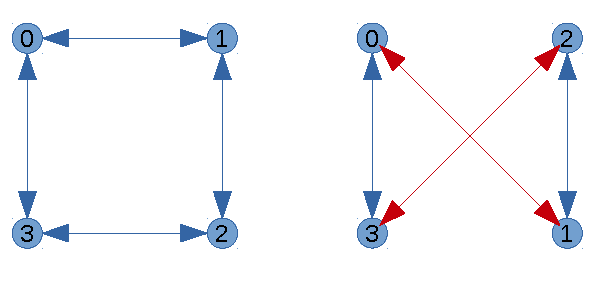
\includegraphics[width=0.475\textwidth]{skewed_layout_cropped.pdf}
  \caption{Skewed layout for 4 Nodes in 1D}
    \label{fig:Skewed_layout_for_4_Nodes_in_1D}
\end{figure}

\subsection{Random Mapping}
\label{sect:random}

Random mappings are generated by using the linux shuf utility to shuffle a regular mapping file.
Since the mappings are random we would expect the average distance between nodes to be close to half the diameter
or the maximum distance between any two nodes in the network. The random mappings generated for a partition of
dimensions 4x4x4x4x2 with 16 ranks per node have an average distance of 4.5. The diameter of network, is the maximum
distance possible between any two nodes in the topology and is the sum of the halves of the length of each dimension: 9.
The maximum distance measured for the mapping file generated is 9.
Despite the increased average distance, the neighbor pairs in a random mapping are randomly distributed over the 5 dimensions and in +/- directions.
While we expect the longer average distance to overall have a negative
effect on performance, the distribution of neighbors along multiple
dimensions could have somewhat of a compensating positive effect
because of the high number of alternative routes between neighbors
and the ability to distribute traffic across all dimensions of the network.

\subsection{Deoptimized Mappings from Simulated Annealing}
In order to cover an even wider range of mappings, we tried to
devise mappings that were worse than the random mapping.
We can obtain an absolute upper bound on average distance of
$9$, because the maximum possible distance in a 5D torus
partition of 4x4x4x4x2 is 9.  It is unclear to us whether
mappings with average distance of $9$ exist, and under what
circumstances they might exist: we were unsuccessful in
attempts to reduce this upper bound.  We were also
unsuccessful in directly devising mappings
with average distance significantly greater than the $\sim4.5$ average
distance obtained with random mapping.

In order to discover mappings with high average distance, we used
a heuristic optimization algorithm that began with a random mapping
and made incremental modifications in an attempt to discover mappings
with higher average distance.
We selected to use simulated annealing~\cite{Press2007} because of the
simplicity and effectiveness of this family of heuristics.

A simulated annealing optimization run starts with aggressive exploration
of the search space, where large perturbations are made and negative
moves are sometimes accepted to allow the algorithm to escape local
minima of the function being optimized.  Over time, the algorithm
transitions to fine-tuning, with smaller perturbations made and negative moves
accepted less frequently.  Pseudocode for the algorithm is shown in
Figure~\ref{fig:anneal_pseudocode}.

\begin{figure}
  {\footnotesize
  \begin{lstlisting}[frame=lines, basicstyle=\ttfamily,columns=fixed]
mapping := random_mapping(app_topo, net_topo)
dist := average_distance(mapping)
for i = 1 to niters do
  temp := calc_temp(i, niters)
  nswaps := calc_swaps(temp, nranks)
  new_mapping := random_swap(mapping, nswaps)
  new_dist := avg_dist(new_mapping)
  if new_dist > dist or
     accept(dist, new_dist, temp) then
    mapping := new_mapping
    dist := new_dist
  end
end
  \end{lstlisting}
  }
  \caption{Pseudocode halo exchange algorithm with concurrent sends and
           receives to all neighbours.}
    \label{fig:anneal_pseudocode}
\end{figure}

The algorithm has several inputs and has several sub-procedures,
which we will describe informally.
\texttt{niters} is the number of annealing iterations to attempt, while
\texttt{app\_topo} and \texttt{net\_topo} are data structures
describing the application and network topology, respectively.

\texttt{random\_mapping} initializes a random mapping, as described
in Section~\ref{sect:random} using the topology information.
\texttt{avg\_dist} computes the average distance between
application neighbors (i.e. ranks that exchange messages in
halo exchange) for the mapping.

\texttt{random\_swap} randomly selects \texttt{nswaps} pairs of ranks
and swaps them, with \texttt  The \texttt{calc\_swaps} function computes
the number of ranks to swap up to 2\% of ranks, swapping more at higher
temperatures:
$$calc\_swaps(temp, nranks) = max(1, \lfloor 0.02 * temp * nranks \rfloor)$$

The \texttt{calc\_temp} function returns a temperature that
decreases from 1 to 0 during the course of the annealing process.
The basic trajectory followed is cubic decrease: $(1 - i/niters)^3$.
Additional cycles of raising and lowering the temperature are also
applied to diverge from this basic trajectory.

\texttt{accept} decides whether to accept a mapping that has lower
average distance, which can the algorithm escape a local maximum.
This is randomized based on a random value $p$ between 0 and 1.
The new mapping is accepted if:
$$temp * (0.5 - (1.0 - new\_dist/dist) * 25) > p$$

Using this approach for upwards of 1 million iterations,
we were able to produce mappings that had average distance substantially
higher than the randomized mapping, although still short of our upper
bound of $9$.  We obtained an average distance of 6.10 and 6.03 for the 5D application and
3D application respectively.

\subsection{Topology-aware Box Partitioned Mapping}

The box partitioned mapping is designed with the goal of placing N-dimensional slices of the application domain on nodes such that
intranode messaging is maximised. This should in turn reduce network traffic and increase overall performance.
We break down the application domain to multi-dimensional slices and place them on adjacent nodes in the network so that that the
overall distance the traffic that exits the node has to travel is minimised. The size and dimensionality of the box is informed
by the network topology and the application domain.

For an application with a 3D domain decomposition of 32x32x8, the box is determined to be 4x2x2. We partition the application domain
into 512 contiguous 3D slices of dimensions 4x2x2. Now, there are 512 boxes arranged as 8x16x4 (32x32x8/4x2x2).
The 512 slices are then mapped on to the 4x4x4x4x2 network topology of the BlueGene/Q.

Sample from the mapping for 3D application of dimensions 32x32x8 to network of dimension 4x4x4x4x2x16:
\begin{lstlisting}[frame=lines, basicstyle=\ttfamily,columns=fixed]
0 0 0 0 0 0
0 0 0 0 0 1
0 0 1 0 0 0
0 0 1 0 0 1
0 0 2 0 0 0
0 0 2 0 0 1
0 0 3 0 0 0
0 0 3 0 0 1
\end{lstlisting}

For an application with a 5D domain decomposition of 8x8x8x8x2, the box is determined to be 2x2x2x2x1. Similar to the 3D case, we
partition the application domain into 512 contiguous into  slices of dimensions 2x2x2x2x1.
Now, there are 512 boxes arranged as 4x4x4x4x2 (8x8x8x8x2/2x2x2x2x1). There is a simple one to one mapping from the
to that of the 4x4x4x4x2 network topology since the dimensionality matches exactly. The difference between the mapping
generated by this method and the regular mapping stems from the mismatch of dimensions in the application domain to that
of the network topology.

Sample from the mapping for 5D application of dimensions 8x8x8x8x2 to network of dimension 4x4x4x4x2x16:
\begin{lstlisting}[frame=lines, basicstyle=\ttfamily,columns=fixed]
0 0 0 0 0 0
0 0 0 0 1 0
0 0 0 0 0 1
0 0 0 0 1 1
0 0 0 1 0 0
0 0 0 1 1 0
0 0 0 1 0 1
0 0 0 1 1 1
\end{lstlisting}

\subsection{Metrics for Measuring a Mapping}

In the earlier sections we have introduced several different mapping strategies, each with different characteristics which could
impact the network performance. To relate the impact of a mapping on network performance it is important to device a metric that
captures the aspects of a mapping that could affect the network. Mappings determine the amount of intranode communication versus
the communication that must go over the network, and over what links these communication occurs.

When message sizes are small and deterministic routing
protocol are in place, a deterministic path with the manhattan distance
between neighbors is chosen.  More interesting network effects become apparent only when message sizes increase. Once message sizes exceed 4Kb, the
rendezvous protocol is used by the network which selects dynamically between
multiple network paths in an attempt to avoid hot-spots.  This can improve load balance between links and
increase network utilization at the cost of
increased latency.
%Since it is difficult to model these dynamic systems, we will not attempt
%to exactly model the routing protocol, but instead assume that it
%balances the network load somewhat evenly such that the number of
%messages flowing over every link does not diverge too much from
%the average.

In all cases, the number of network hops between neighbors has a
direct effect on the probability that a message sent between the
neighbors will contend for a link with another message.
Average distance is thus a way of summarizing a mapping that will
directly influence its performance.
The average distance between neighbors can easily be calculated by taking the average of the manhattan distance of all pairs of neighbors.
We assume that the distance between two ranks on the same node is 0, since intranode messaging does not contribute to network traffic.
This average distance \textbf{N\textsubscript{steps}}, can now be treated as a proxy for average network traffic flowing over any particular.


Let the torus network be of \textbf{D} dimensions, and let \textbf{N\textsubscript{ranks}} be the number of ranks in the partition.
The total logical neighbors involved in halo exchange is :
\begin{equation}
  N_{neighbors} = N_{ranks} * 2 * D
\end{equation}

For every rank 0 $<$ \textbf{u} $<$ \textbf{N\textsubscript{ranks}}, the neighbors of u are \textbf{neighbors(u)},then the manhattan distance
between every pair of neighbors is calculated by the distance function \textbf{dist\textsubscript{(u,v)}}.
The average number of messages flowing through any link is given by:

\begin{equation}
  N_{steps} = \frac{ \sum\limits^{N_{ranks} - 1}_{u \mathop =0} \sum\limits_{v\in{neighbors(u)}} dist_{u,v}  }  {N_{neighbors}}
  %N_{steps} = \frac{ \sum_{u \mathop =1}^{N_{ranks}} \sum\limits_{v\in{neighbors(u)}} dist_{u,v} } {N_{neighbors}}
\end{equation}



The average distance for the various mappings for the 3D and 5D case are provided in table


\begin{table}
  \caption{Average distance for mappings from 8x8x8x8x2 domain to 4x4x4x4x2x16 topology}
  {\footnotesize
    \begin{tabular}{| l | l | p{1.5cm} |}
    \hline
    Mapping         & Avg. Distance & Max Dist\\ \hline
    regular         & 1.050000 & 3.000000\\ \hline
    linear          & 1.450000 & 3.000000\\ \hline
    reversed        & 1.450000 & 3.000000\\ \hline
    random          & 4.504980 & 9.000000\\ \hline
    skewed regular  & 1.100000 & 3.000000\\ \hline
    skewed reversed & 1.450000 & 3.000000\\ \hline
    optimized       & 0.600000 & 1.000000\\ \hline
    de-optimized    & 6.106348 & 9.000000\\ \hline
    \hline
    \end{tabular}
  }
\end{table}


\begin{table}
  \caption{Average distance for mappings from 32x32x8 domain to 4x4x4x4x2x16 topology}
  {\footnotesize
    \begin{tabular}{| l | l | p{1.5cm} |}
    \hline
    Mapping         & Avg. Distance & Max Dist\\ \hline
    regular         & 1.145833 & 4.000000\\ \hline
    linear          & 1.625000 & 4.000000\\ \hline
    reversed        & 1.625000 & 4.000000\\ \hline
    random          & 4.499023 & 9.000000\\ \hline
    skewed regular  & 0.979167 & 4.000000\\ \hline
    skewed reversed & 1.645833 & 4.000000\\ \hline
    optimized       & 0.479167 & 2.000000\\ \hline
    de-optimized    & 6.530436 & 9.000000\\ \hline
    \hline
    \end{tabular}
  }
\end{table}


\section{Analytical Model for Network Communication}\label{sect:model}

There are a wide range of possible models that could be used to
estimate network communication performance for a complex network
such as those on BlueGene/Q or Cray XE6.  These models range from
full-fidelity simulations that directly simulate packet routing, to
simplified models that estimate performance based on simplified
assumptions.  These simplified models are often very useful for
understanding and prediction, but typically have a limited domain
of applicability.  For example, network models that ignore congestion
can be suitable for modeling single point-to-point transfers, but are
unsuitable for modeling many simultaneous transfers over a shared network.

For halo exchange, we need a model that captures multiple
simultaneous data transfers contending for shared resources: we
expect that many of these messages will need to transit the
same network links.  We can, however, simplify the model by exploiting the
symmetry of the communication pattern, in which each MPI rank sends
and receives the same amount of data. For this reason, we choose a
model that assumes that traffic is distributed fairly evenly
throughout the network and that communication throughput is limited
by the aggregate capacity of the network's links.

We arrived at our model for Time to completion \textbf{T} based on two assumptions.
We first assume that the limiting factor on transfer throughput will be
the most trafficked link on the network - the one that the most bytes
must transit during the halo exchange.  Finding the most trafficked
link and determining the number of bytes transferred is not feasible for our
simple model, because it would require simulating network load and
the Blue Gene/Q adaptive routing algorithms. We make a second assumption
that traffic is distributed fairly evenly across the network because of
the halo exchange pattern and adaptive routing, the maximum number of bytes
transiting a link will be closely correlated with the average number of bytes transiting a link.

On an HPC system such as BlueGene/Q or Cray XE6, each node has multiple duplex links to it's neighbors.
If the application on every node attempts to exchange messages with every neighbor, we can assume that
every link on the network will see similar traffic. Thus we, consider a single link and it's bandwidth
to determine \textbf{t\textsubscript{b}} the time required to send a Byte along the link.
Assume that there are \textbf{N\textsubscript{procs}} number of identical processes all of which will attempt to utilize the same links.
To capture the differences between different mappings we calculate the average distance between neighbors,
\textbf{N\textsubscript{steps}}. We have implemented a program in Python that
takes a BlueGene/Q mapping file and computes the average distance in
a halo exchange computation based on the application domain decomposition
and the network topology of a Blue Gene/Q partition.

The current MPI implementation on leadership class systems like Mira (Bluegene/Q) utilizes
shared memory for intranode communication. When a neighbor is present within the same node, the link
is weighted as zero, and every network link or hop is weighted as one. Since it is possible to place
neighboring tasks from the application domain on the same node there are mappings possible which
minimize N\textsubscript{steps} below one. There are constant costs involved in startup, acquiring a buffer etc,
and t\textsubscript{c} represents the various constant costs
of network communication using MPI.  N is the message size in bytes that are exchanged between neighbors.

From our understanding of the constant consts of communication involved in different of MPI messaging protocols,
we can consider t\textsubscript{c} will vary for different message sizes. As a result t\textsubscript{c} will
be calibrated from a halo exchange workload at datasizes close to the thresholds between the 4 protocols.
The models will be required to use the t\textsubscript{c} for the protocol which would be used for the datasizes
being sent. The thresholds for the protocols are listed in Table~\ref{table:bgq_protocols}.

The network load balancing provided by the rendezvous protocol is expected to
be imperfect, and will be unable to saturate all network links.  We will use an experimentally calibrated constant \textbf{$\alpha$}
to account for this unused network capacity.

A simple analytical model determines the time to completion, T of a complete halo exchange operation,
from the variables defined above as follows:
\begin{equation}
  T = t_c + (N_{steps} * N_{procs} * N * t_b * \alpha)
\end{equation}


\section{Experimental Design}\label{sect:experimental design}

Empirical studies are necessary to gauge the accuracy of models. Considerable efforts have
been taken to ensure that the experiments are fair and are an accurate reproduction of the Halo exchange pattern
in real world scenarios. The experiments have been repeated multiple times on different partitions on the machine
to ensure that partition-specific effects do not influence results.
We have not attempted to reproduce results on different machines
of the same architecture due to time limitations, but we have no
reason to expect significantly different results.

\begin{figure*}[ht]
  {\footnotesize
  \begin{lstlisting}[frame=lines, basicstyle=\ttfamily,columns=fixed]
MPI_Comm comm_cart
MPI_Request req[4*N_dims]

for dim = 1 to N_dims do:
    MPI_Cart_Shift (comm_cart, dim,  1, rank_src[0][dim], rank_dst[0][dim]
    MPI_Cart_Shift (comm_cart, dim, -1, rank_src[1][dim], rank_dst[1][dim]
end

MPI_Barrier(comm_cart)
halo_timer(begin)
for dim = 1 to N_dims do
    # Send/recv message along dim+
    MPI_Isend(send_buffer, datalength, destination_ranks[0][dim], comm_cart, req[i*4])
    MPI_Irecv(send_buffer, datalength, source_ranks[0][dim], comm_cart, req[i*4+1])
    # Send/recv message along dim-
    MPI_Isend(send_buffer, datalength, destination_ranks[0][dim], comm_cart, req[i*4+2])
    MPI_Irecv(send_buffer, datalength, source_ranks[0][dim], comm_cart, req[i*4+3])
end

MPI_Waitall(4*N_dims, req)
MPI_Barrier(comm_cart)
halo_timer(end)
  \end{lstlisting}
  }
  \caption{Pseudocode halo exchange algorithm with concurrent sends and
           receives to all neighbours.}
    \label{fig:halo_pseudocode}
\end{figure*}

Since we are only interested in the network performance aspect of the halo exchange code, we only measure
the time taken to complete the halo exchange communication. The pseudocode for the halo exchange is listed in Figure~\ref{fig:halo_pseudocode}.

\subsection{Latency}
On the BlueGene/Q, the latency between the closest node and the farthest node is estimated to be under 3$\mu$s\cite{BGQ_Interconnect_2012,BGQ_RedBook_2013}.
This latency
is negligible compared to the total time to completion of a halo exchange operation. Other authors~\cite{Bhanot_2005} working on Blue Gene/L have suggested
that hop count has a significant effect on latency, but we do not expect
that latency from increased hop count will significantly affect the
performance of halo exchange on the Blue Gene/Q.

Therefore, in the analytical model described in Section~\ref{sect:model}, we assumed that latency does not play a role.
This assumption was experimentally tested by comparing the time to completion of halo exchanged between the default mapping and a modified
mapping which has just two ranks interchanged to nodes that span the diameter of the torus. 
This results in the an increase in maximum distance
from 3.0 to 9.0 and increase of 0.003 for the average distance between neighbors.
Since our halo exchange timings measure the time until all communications
are completed, the entire operation is only as fast as the slowest pairwise
exchange.

\subsection{Cache Effects}
To determine whether the network performance is affected by the send/receive message buffers overflowing from the
L3 caches, we designed an experiment which sent \textbf{DUPES} number of messages each with $\frac{datalength}{DUPES}$
message size. The runs were compared against a run with DUPES=1. 
We expect that the added startup cost associated with the
additional messages will lead to higher time to completion for short messages for
$DUPES>1$.
If L3 cache overflow was limiting halo exchange performance at higher data
sizes, then we would expect that the Halo runs with $DUPES>1$ should outperform
the runs with $DUPES=1$ because of the lower memory footprint.

\subsection{Task Placement within Mappings for 3D and 5D Application Domains}
We've described eight different mapping schemes in Section~\ref{sect:mapping}.
To study the network performance of the halo exchange codes, they are exercised using varying levels of data lengths for message exchanged between neighbors.
Powers of 2 ranging from 8B to 32MB are chosen as data sizes.  This range
covers all Blue Gene/Q MPI messaging protocols and covers
a reasonable swath of data sizes that real world application might use. The hardware partitions chosen are 512 node partitions of 4x4x4x4x2 shape. This
is one rack on the BlueGene/Q, and is large enough to be representative of
real halo exchange applications.

The Halo exchange code itself measures the performance of various blocking and non-blocking MPI send and recv primitives and combinations.
For our experiments we will only consider MPI\_Isend and MPI\_Irecv primitives with no artificial delay introduced after the barrier.
The pseudocode for the halo exchange is listed in Figure~\ref{fig:halo_pseudocode}.
Evaluating the performance of the different MPI primitives with randomised delay options is beyond the scope of this paper.


\begin{figure}
  \center
  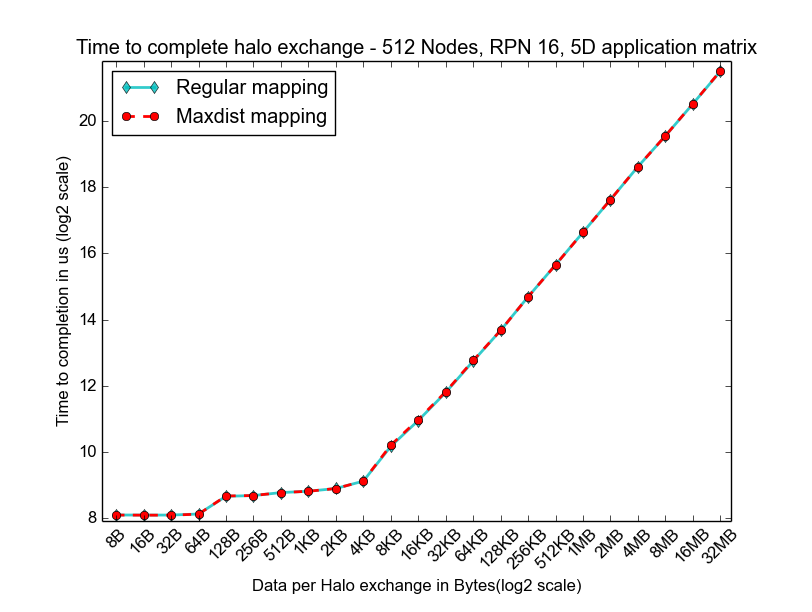
\includegraphics[width=0.45\textwidth]{regular_vs_maxdist.png}
  \caption{Regular mapping and Maxdist mapping}
    \label{fig:regular_vs_maxdist}
\end{figure}


\begin{figure}
  \center
  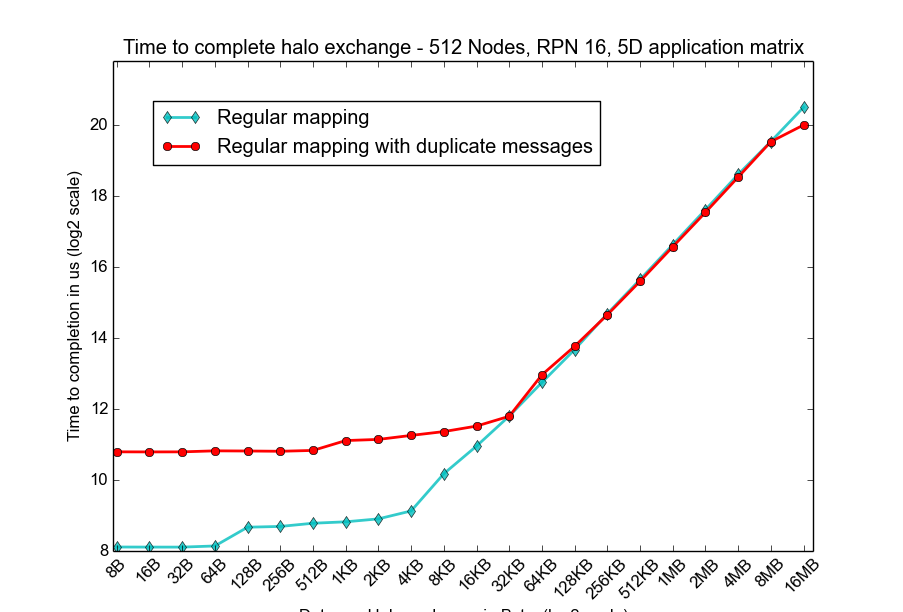
\includegraphics[width=0.45\textwidth]{regular_vs_cache_duplicates.png}
  \caption{Regular mapping with 8 duplicates and without}
    \label{fig:caching_figure_vs_without}
\end{figure}

The analytical model described in Section~\ref{sect:model}, is informed by the nature of the target system
and the domain decomposition of the application. The value of a model is in the ability to predict the
results from
% What machine do we run on
%

\begin{figure}
  \center
  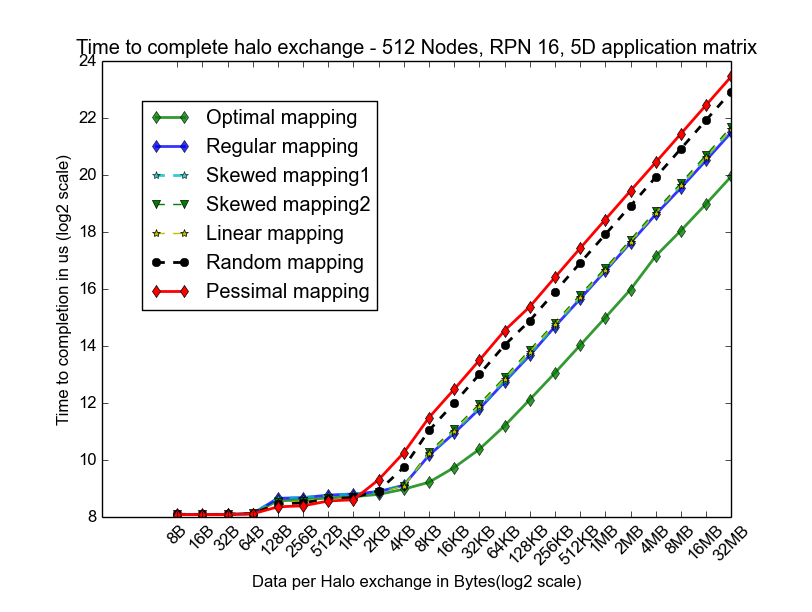
\includegraphics[width=0.45\textwidth]{5D_512_all_mappings.png}
  \caption{5D halo exchange on 512 nodes with 16 RPN}
    \label{fig:5D halo exchange on 512 nodes with 16 RPN}
\end{figure}


\begin{figure}
  \center
  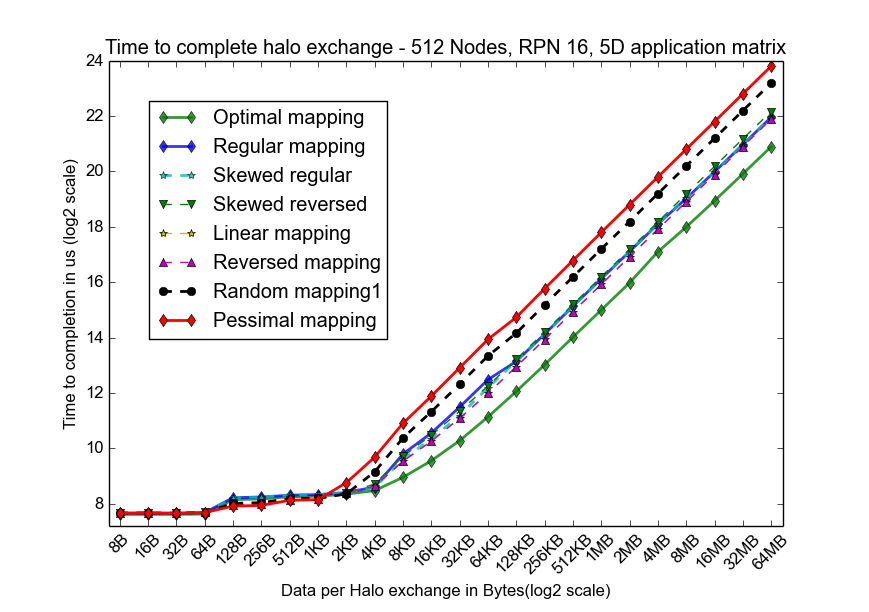
\includegraphics[width=0.45\textwidth]{3D_512_all_mappings.png}
  \caption{3D halo exchange on 512 nodes with 16 RPN}
    \label{fig:3D halo exchange on 512 nodes with 16 RPN}
\end{figure}


\section{Results}

The insights gained from the experiments outlined in Section~\ref{sect:experimental design}
has guided the development of the Analytical model for the performance of halo exchange.
The results from these experiments are described below:

The experiments to study caching effects, show that at higher data sizes the time to completion
is unaffected by using duplicate messages of smaller sizes. If caching effects played any significant
role in performance sending multiple duplicate messages that fit in the L3 cache would have
outperformed larger messages that do not fit in L3 cache. The plots of these two cases are shown
in Figure~\ref{fig:caching_figure_vs_without}. We see that sending duplicate messages of smaller
size has added startup costs but at higher data sizes cache optimized  duplicate messages do not
perform better, from this we conclude that caching effects are negligible and can be ignored.

The latency experiments used a modified regular mapping in which two ranks were transposed to
nodes that are diametrically apart. This introduced a negligible increase in average distance but
increased the maximum distance between neighbors from 3 to 9. The results from this experiment
in Figure~\ref{fig:regular_vs_maxdist} show that increasing the distance does not add any measurable
latency penalty. The results from this experiment contradicts the assumptions used in prior work ~\cite{Bhanot_2005}
that the number of hops involved affect performance directly through increased latency.

Plots of the different mappings discussed in Section~\ref{sect:mapping} indicate that increasing
the halo exchange message length consistently affects performance.
Figure~\ref{fig:5D halo exchange on 512 nodes with 16 RPN} and figure~\ref{fig:3D halo exchange on 512 nodes with 16 RPN}
are plots of all mappings for the 5D application and 3D application respectively.

Analysis of the \% difference between the predictions by the Analytical model and empirical data
for the experiments using 3D and 5D application matrices are shown in Table~\ref{table:data vs model 3d}
and Table~\ref{table:data vs model 5d} respectively. The tables show the minimum and maximum error
as well as the average of the absolute error percentages for message sizes from 8B to 16Mb. For the
3D application, the experimental results differ from the analytical model by 53.60\% in the worst case,
while the average absolute error is under 30\%. The average absolute error is under 20\% with the
maximum divergence being 44.12\% for the 5D application.

Table~\ref{table:optimized vs deoptimized} shows a comparison between the optimized mappings and the
regular mapping, and de-optimized mappings. The optimized mapping yields a 2x performance advantage
over the regular mapping in both the 3D and 5D applications.

\begin{table}
  \caption{Optimized vs De-optimized mapping comparison
    \label{table:optimized vs deoptimized}}
  {\footnotesize
    \begin{tabular}{ | l | l | l | p{1.5cm} |}
    \hline
    \input tables/regular_vs_optimal.tex
    \hline
    \end{tabular}
  }
\end{table}

\begin{table}
  \caption{3D Experimental data vs Analytical model
    \label{table:data vs model 3d}}
  {\footnotesize
    \begin{tabular}{ | l | l | l | p{1.5cm} |}
    \hline
    Mapping    &    Min Error\% &    Max Error\% & Avg abs Error\%\\ \hline
    Optimized  &         -16.63 &          30.88 &         13.17\\ \hline
    Regular    &          -0.49 &          36.68 &         15.31\\ \hline
    Linear     &         -24.12 &          14.00 &         10.91\\ \hline
    Reversed   &         -24.13 &          13.93 &         11.00\\ \hline
    Skewed regular &      -0.39 &          39.57 &         19.81\\ \hline
    Skewed reversed&     -20.52 &          18.44 &          7.04\\ \hline
    Random  &            -53.60 &          23.63 &         27.41\\ \hline
    De-optimized &       -50.07 &          38.67 &         28.79\\ \hline
    \hline
    \end{tabular}
  }
\end{table}


\begin{table}
  \caption{5D Experimental data vs Analytical model
    \label{table:data vs model 5d}}
  {\footnotesize
    \begin{tabular}{ | l | l | l | p{1.5cm} |}
    \hline
    Mapping         &    Min Error\% &   Max Error\% & Avg abs Error\%\\ \hline
    Optimized       &         -44.12 & 16.01 & 15.88\\ \hline
    Regular         &         -0.41  & 32.42 & 17.07\\ \hline
    Skewed regular  &         -0.68  & 30.98 & 16.96\\ \hline
    Skewed reversed &         -9.31  & 17.69 & 8.99\\ \hline
    Linear          &         -9.44  & 17.20 & 6.71\\ \hline
    Reversed        &         -9.36  & 17.12 & 6.64\\ \hline
    Random          &         -35.86 & 35.19 & 15.69\\ \hline
    De-optimized    &         -27.84 & 50.24 & 14.96\\ \hline
    \hline
    \end{tabular}
  }
\end{table}

\begin{figure}
  \center
  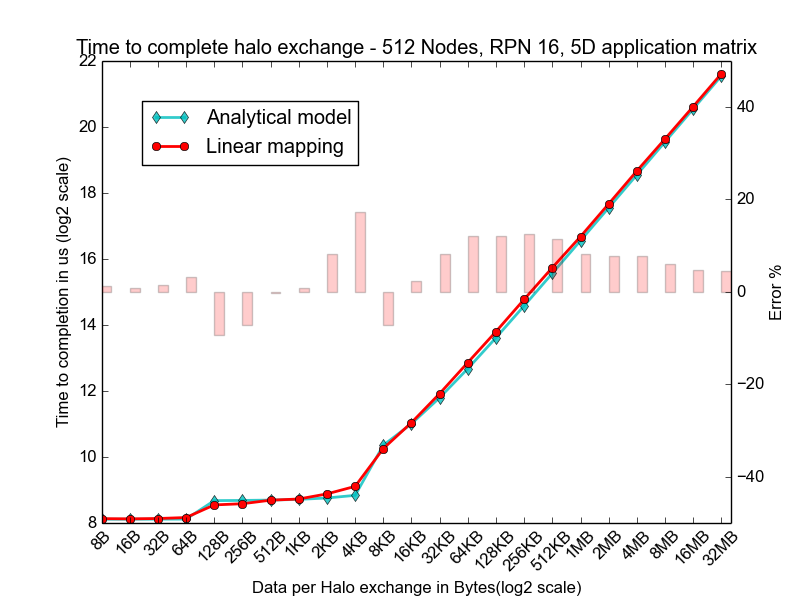
\includegraphics[width=0.45\textwidth]{mappings/5d_linear_model.png}
  \caption{Analytic model vs Experimental data for Linear mapping(5D)}
    \label{fig:5D_linear_mapping}
\end{figure}


\begin{figure}
  \center
  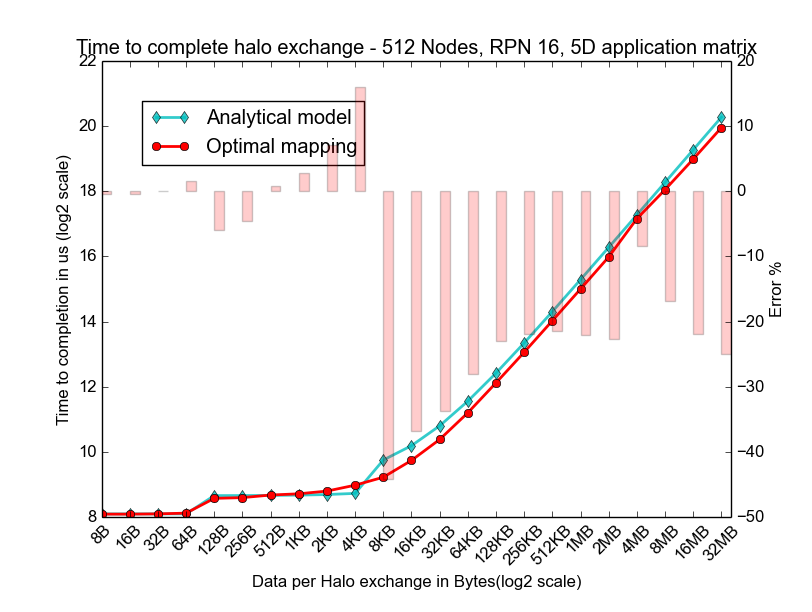
\includegraphics[width=0.45\textwidth]{mappings/5d_optimal_model.png}
  \caption{Analytic model vs Experimental data for Optimal mapping(5D)}
    \label{fig:5D_optimal_mapping}
\end{figure}

\begin{figure}
  \center
  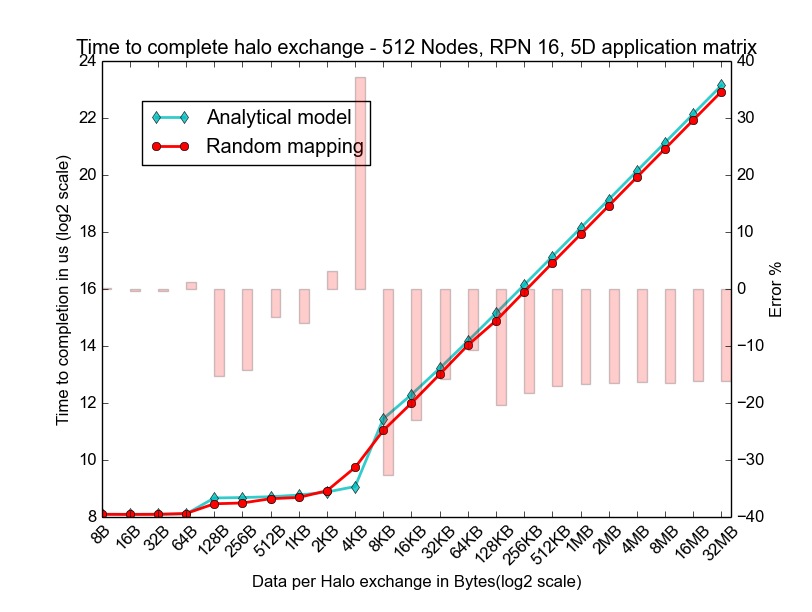
\includegraphics[width=0.45\textwidth]{mappings/5d_random_model.png}
  \caption{Analytic model vs Experimental data for Random mapping(5D)}
    \label{fig:5D_random_mapping}
\end{figure}

\begin{figure}
  \center
  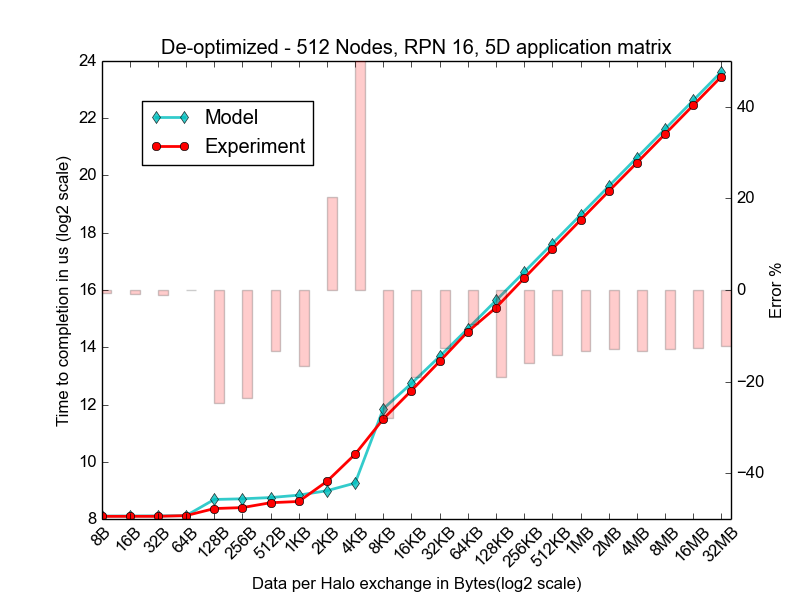
\includegraphics[width=0.45\textwidth]{mappings/5d_pessimal.png}
  \caption{Analytic model vs Experimental data for De-optimized mapping(5D)}
    \label{fig:5D_pessimal_mapping}
\end{figure}

\begin{figure}
  \center
  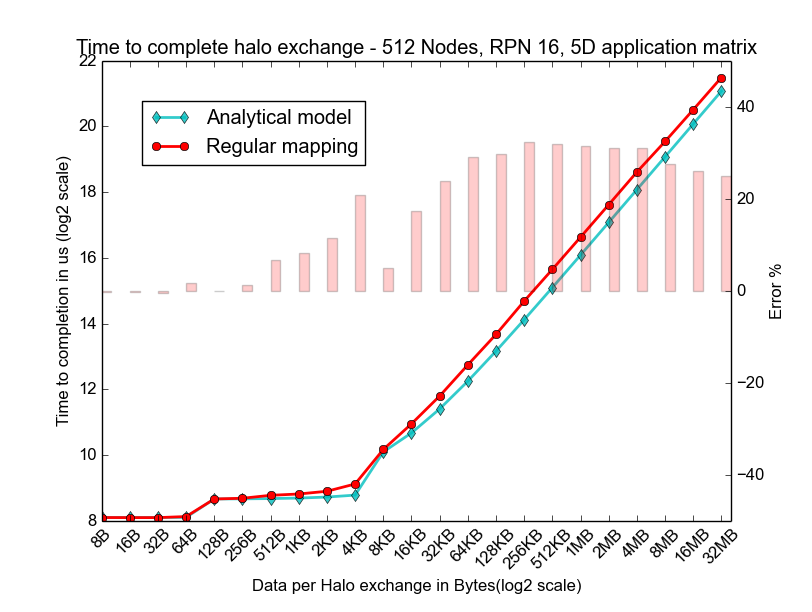
\includegraphics[width=0.45\textwidth]{mappings/5d_regular_model.png}
  \caption{Analytic model vs Experimental data for Regular mapping(5D)}
    \label{fig:5D_regular_mapping}
\end{figure}

\begin{figure}
  \center
  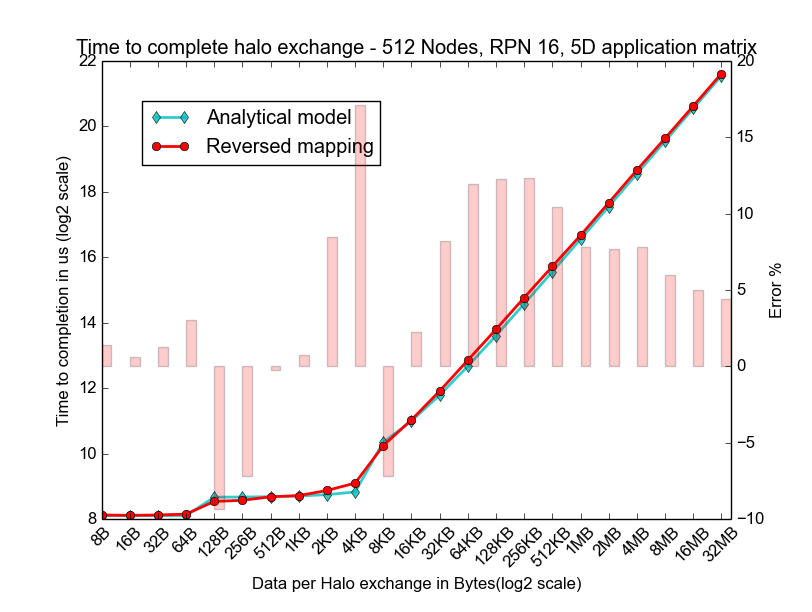
\includegraphics[width=0.45\textwidth]{mappings/5d_reversed_model.png}
  \caption{Analytic model vs Experimental data for Reversed mapping(5D)}
    \label{fig:5D_reversed_mapping}
\end{figure}

\begin{figure}
  \center
  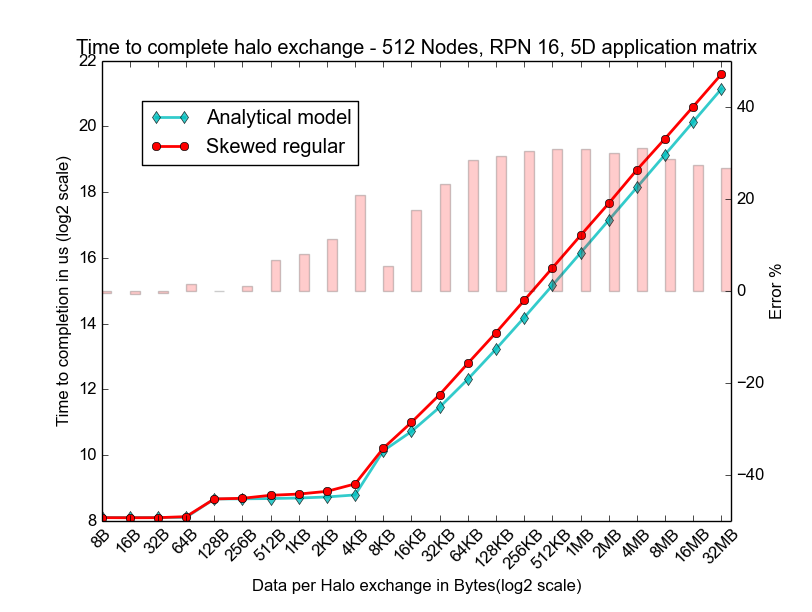
\includegraphics[width=0.45\textwidth]{mappings/5d_skewed_regular.png}
  \caption{Analytic model vs Experimental data for Skewed regular mapping(5D)}
    \label{fig:5D_skewed_regular_mapping}
\end{figure}

\begin{figure}
  \center
  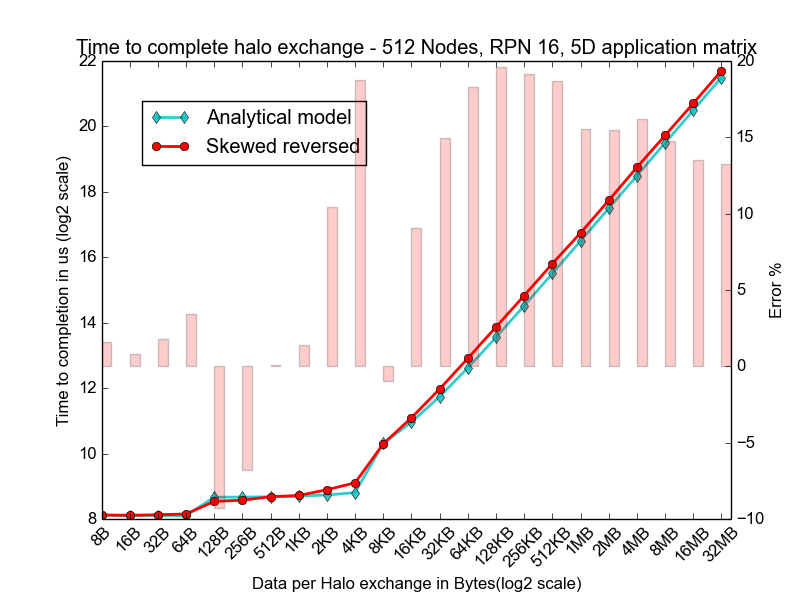
\includegraphics[width=0.45\textwidth]{mappings/5d_skewed_reversed.png}
  \caption{Analytic model vs Experimental data for Skewed reversed mapping(5D)}
    \label{fig:5D_skewed_reversed_mapping}
\end{figure}

\section{Conclusion}

We have conducted a detailed study of the impact of task placements on Halo exchange
style operations on the Blue Gene/Q. From the insights gained from these experiments
we developed an analytical model and a metric to compare different mapping schemes.
The experimental studies show that the average prediction error of the model for any
given mapping is under 30\%.

We explored several different mapping strategies, and compared results against the model.
These mappings include an optimized mapping which is close to the theoretical optimum,
and a de-optimized mapping generated using simulated annealing. The results from these
different mappings show that performance can vary widely, with the optimized mapping
being 7.5 times faster than the de-optimezed mapping. The optimized mapping also out-performs
the default mapping scheme for the 3D application by 2.0x and the 5D application
by 2.6x in the rendezvous protocol regime.

To further the understanding of this model and to validate the effectiveness of the model,
similar experiments must be conducted on other network architectures such as the Cray XE6, a 3D torus.
We believe that experiments on other architectures will yield a better understanding of the model
as well as ensure the applicability of the model in different environment. Our tests show that
latency does not impact performance on the Blue Gene/Q, but this might not be true on other networks
and architectures. Currently we have very little understanding of the experimentally calibrated
link utilization parameter $\alpha$. Further experiments and studies would help understand what
contributes to this parameter which reduces network utilization considerably.

Improving the model beyond using average distance, which captures the average flow, rather than
the traffic flow over the most congested links can possibly improve error percentages. The average
distance does not capture network hotspots and communication patterns that heavily congest certain
links which effectively reduces available bandwidth. This is a limitation of the model that can be
improved upon.

When halo exchanges involve more complex communication patterns, such as when the neighbors
are a graph pattern, the method discussed using simulated annealing could be used to generate
optimized mappings. Using simulated annealing to generate optimized mapping for our current applications
is also another area where future work is warranted.

\begin{figure}
  \center
  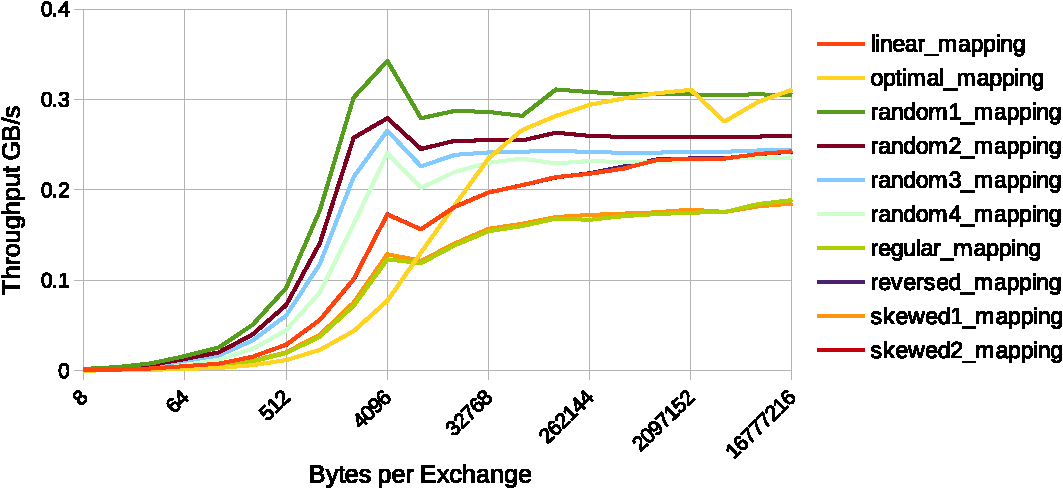
\includegraphics[width=0.45\textwidth]{fig/TEST_RPN_16_NODE_512_5D_LINK_UTIL}
  \caption{Average link utilization during 5D Halo exchange for different
          mappings
    \label{fig:TEST_RPN_16_NODE_512_5D_LINK_UTIL}}
\end{figure}


\begin{figure}
  \center
  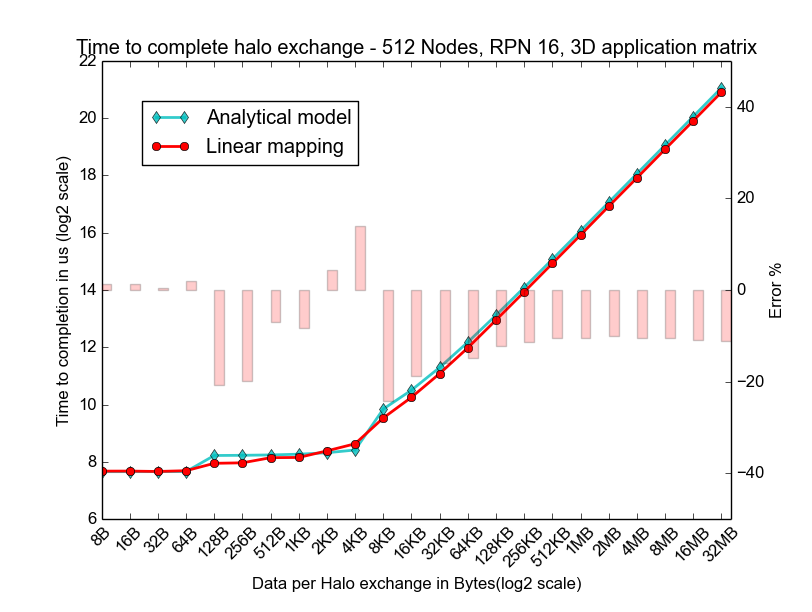
\includegraphics[width=0.45\textwidth]{mappings/3d_linear.png}
  \caption{Analytic model vs Experimental data for Linear mapping(3D)}
    \label{fig:3D_linear_mapping}
\end{figure}

\begin{figure}
  \center
  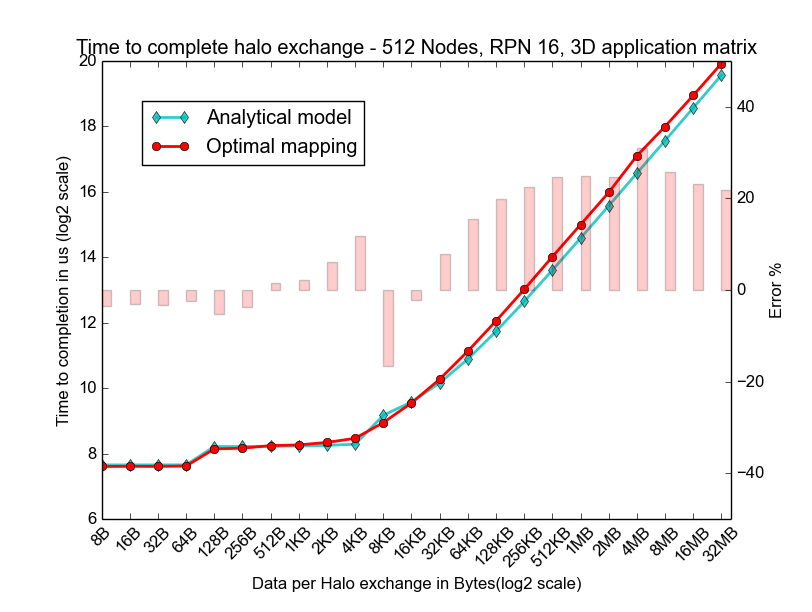
\includegraphics[width=0.45\textwidth]{mappings/3d_optimal.png}
  \caption{Analytic model vs Experimental data for Optimal mapping(3D)}
    \label{fig:3D_optimal_mapping}
\end{figure}

\begin{figure}
  \center
  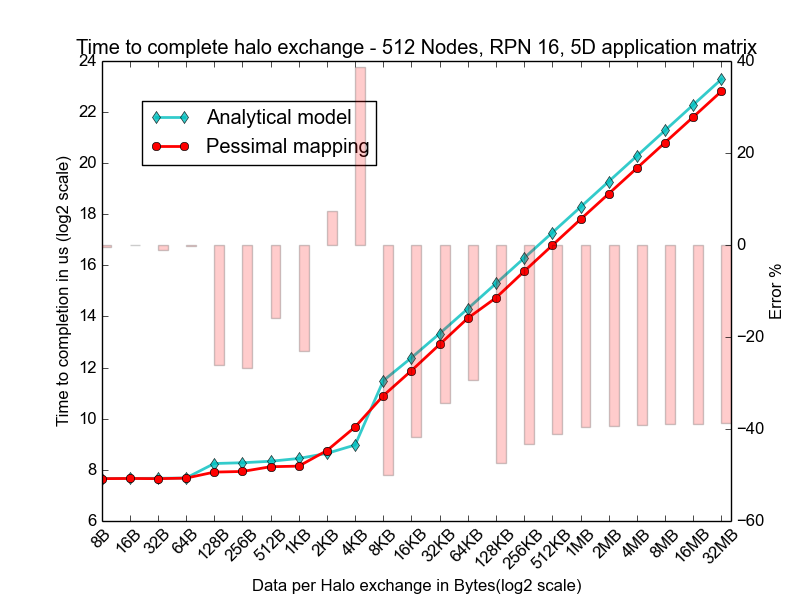
\includegraphics[width=0.45\textwidth]{mappings/3d_pessimal.png}
  \caption{Analytic model vs Experimental data for Pessimal mapping(3D)}
    \label{fig:3D_pessimal_mapping}
\end{figure}

\begin{figure}
  \center
  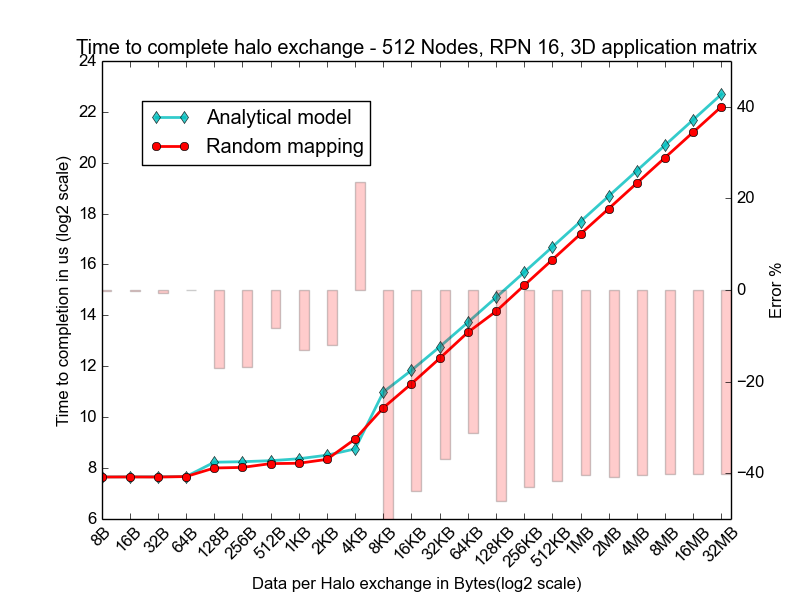
\includegraphics[width=0.45\textwidth]{mappings/3d_random.png}
  \caption{Analytic model vs Experimental data for Random mapping(3D)}
    \label{fig:3D_random_mapping}
\end{figure}

%\clearpage
\begin{figure}
  \center
  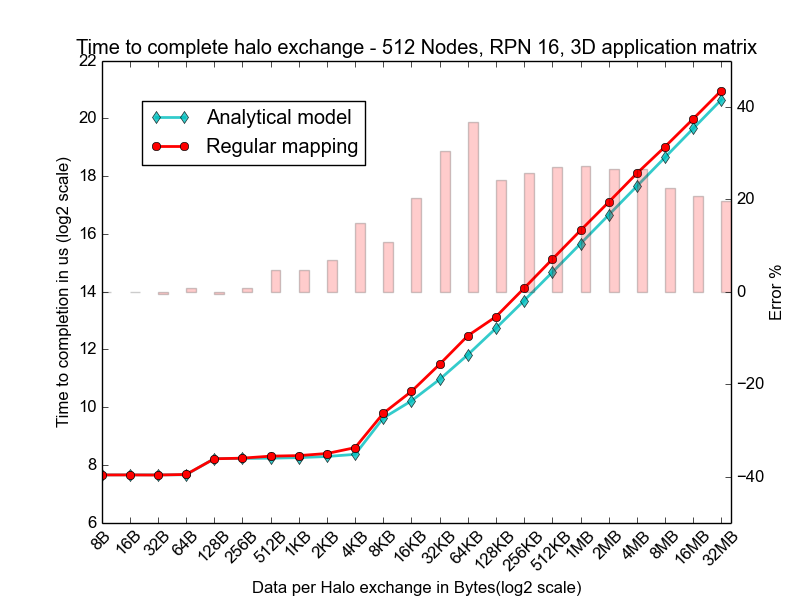
\includegraphics[width=0.45\textwidth]{mappings/3d_regular.png}
  \caption{Analytic model vs Experimental data for Regular mapping(3D)}
    \label{fig:3D_regular_mapping}
\end{figure}

\begin{figure}
  \center
  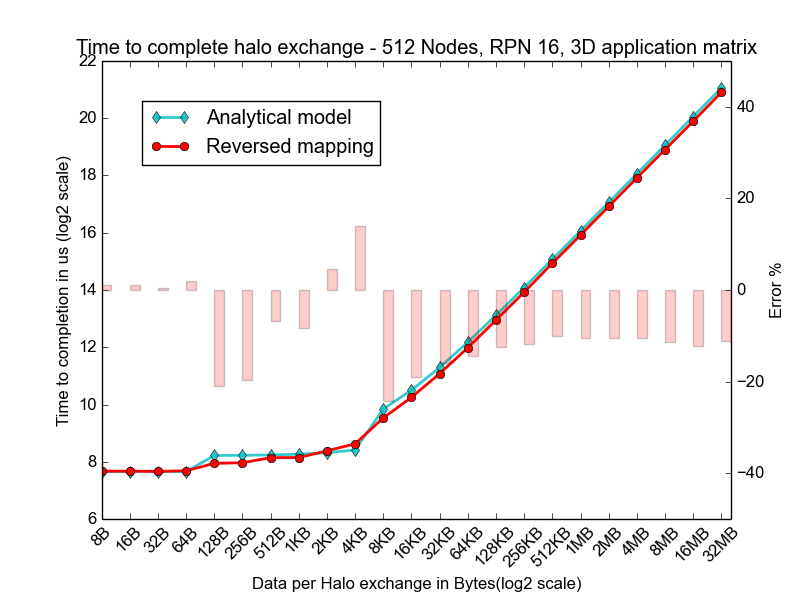
\includegraphics[width=0.45\textwidth]{mappings/3d_reversed.png}
  \caption{Analytic model vs Experimental data for Reversed mapping(3D)}
    \label{fig:3D_reversed_mapping}
\end{figure}

\begin{figure}
  \center
  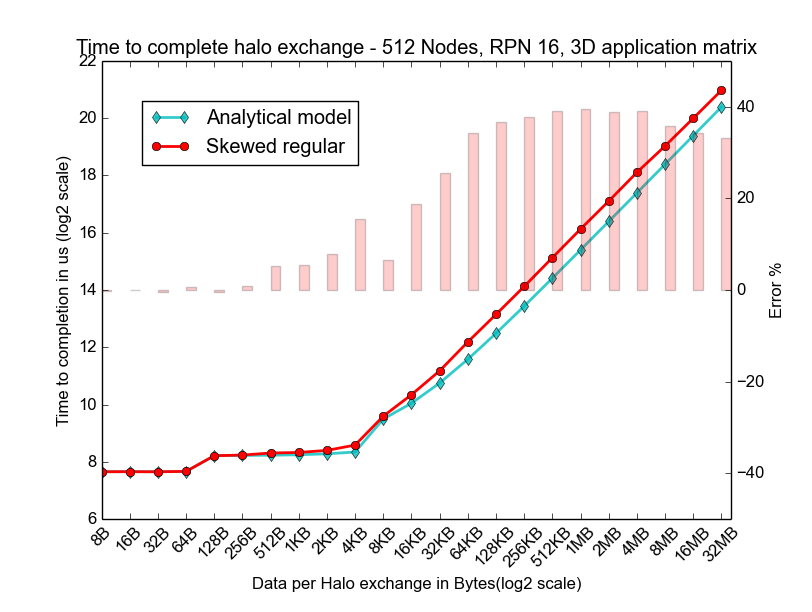
\includegraphics[width=0.45\textwidth]{mappings/3d_skewed_regular.png}
  \caption{Analytic model vs Experimental data for Skewed regular mapping(3D)}
    \label{fig:3D_skewed_regular}
\end{figure}

\begin{figure}
  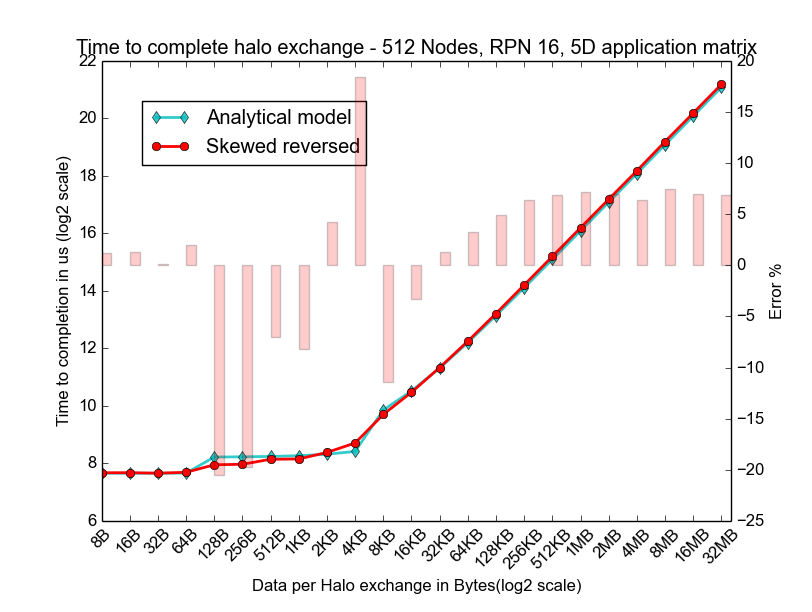
\includegraphics[width=0.45\textwidth]{mappings/3d_skewed_reversed.png}
  \caption{Analytic model vs Experimental data for Skewed reversed mapping(3D)}
    \label{fig:3D_skewed_reversed}
\end{figure}

\bibliographystyle{abbrv}
\bibliography{halo}

\end{document}
